\section{\texttt{rstanarm} e \texttt{brms}}

\subsection{Leituras Recomendadas}
\begin{frame}{\texttt{rstanarm} e \texttt{brms} - Leituras Recomendadas\footnote{\texttt{rstanarm} - \url{http://mc-stan.org/rstanarm/} e \texttt{brms} - \url{https://paul-buerkner.github.io/brms/}}}
	\begin{vfilleditems}
		\item Vinheta e Manual do \texttt{rstanarm} de \textcite{rstanarm}
		\item Vinheta e Manual do \texttt{brms} de \textcite{brms}
		\item Tutorial de \texttt{rstanarm} de \textcite{muth2018user}
		\item Tutorial de \texttt{brms} de \textcite{burknerAdvancedBayesianMultilevel2018}
		\item \textit{Workflow} Bayesiano de \textcite{gelmanBayesianWorkflow2020}
		\item \textit{Workflow} Visual Bayesiano de \textcite{gabryVisualizationBayesianWorkflow2019}
		\item Vinheta e Manual do \texttt{bayesplot} \textcite{bayesplot}
		\item \textcite{storopoli2021estatisticabayesianaR} - \texttt{rstanarm} e \texttt{brms}
	\end{vfilleditems}
\end{frame}

\subsection{Ecosistema \texttt{Stan}}
\begin{frame}{O que é \href{https://mc-stan.org}{\texttt{Stan}}}
	\begin{columns}
		\begin{column}{0.8\textwidth}
			\href{https://mc-stan.org}{\texttt{Stan}}
			\parencite{carpenterStanProbabilisticProgramming2017} é uma \textbf{plataforma para
				modelagem e computação estatística de alto desempenho}.
			Milhares de usuários contam com \texttt{Stan} para modelagem estatística,
			análise de dados e previsão nas ciências sociais, biológicas e físicas,
			engenharia e negócios.
		\end{column}
		\begin{column}{0.2\textwidth}
			\centering
			\includegraphics[width=0.6\textwidth]{stan_transparent.png}
		\end{column}
	\end{columns}
\end{frame}

\subsubsection{Interfaces Oficiais}
\begin{frame}{Interfaces do \href{https://mc-stan.org}{\texttt{Stan}}}
	\begin{vfilleditems}
		\item \texttt{R}: \href{https://mc-stan.org/users/interfaces/rstan.html}{\texttt{RStan}} e \href{https://mc-stan.org/cmdstanr}{\texttt{CmdStanR}}
		\item Python: \href{https://mc-stan.org/users/interfaces/pystan.html}{\texttt{PyStan}} e \href{https://cmdstanpy.readthedocs.io/en/latest/getting_started.html}{\texttt{CmdStanPy}}
		\item \texttt{Shell} (Linha de Comando): \href{https://mc-stan.org/users/interfaces/cmdstan.html}{\texttt{CmdStan}}
		\item \texttt{Julia}: \href{https://mc-stan.org/users/interfaces/julia-stan.html}{\texttt{Stan.jl}}
		\item \texttt{Scala}: \href{https://github.com/cibotech/ScalaStan}{\texttt{ScalaStan}}
		\item \sout{\texttt{Matlab}}: \href{https://mc-stan.org/users/interfaces/matlab-stan.html}{\sout{\texttt{MatlabStan}}}
		\item \sout{\texttt{Stata}}: \href{https://mc-stan.org/users/interfaces/stata-stan.html}{\sout{\texttt{StataStan}}}
		\item \sout{\texttt{Mathematica}}: \href{https://mc-stan.org/users/interfaces/mathematica-stan.html}{\sout{\texttt{MathematicaStan}}}
	\end{vfilleditems}
\end{frame}

\begin{frame}{Interfaces Amigáveis do \href{https://mc-stan.org}{\texttt{Stan}}}
	Somente para \texttt{R}
	\begin{columns}
		\begin{column}{0.8\textwidth}
			\begin{vfilleditems}
				\item \href{http://mc-stan.org/rstanarm/}{\texttt{rstanarm}} \parencite{rstanarm}: ajuda o usuário a especificar modelos usando a sintaxe familiar de fórmulas do \texttt{R}.
				\item \href{https://paul-buerkner.github.io/brms/}{\texttt{brms}} \parencite{brms}: similar ao \texttt{rstanarm} pois usa a sintaxe familiar de fórmulas do \texttt{R}, mas dá maior flexibilidade na especificação de modelos mais complexos.
			\end{vfilleditems}
		\end{column}
		\begin{column}{0.2\textwidth}
			\centering
			\includegraphics[width=0.6\textwidth]{brms.png}
		\end{column}
	\end{columns}
\end{frame}

\begin{frame}[fragile]{Código \href{https://mc-stan.org}{\texttt{Stan}}}
	\begin{lstlisting}[basicstyle=\small, language=Stan]
    data {
      int<lower=0> N;
      vector[N] x1;
      vector[N] x2;
      vector[N] y;
    }
    parameters {
      real alpha;
      vector[2] beta;
      real<lower=0> sigma;
    }
    model {
      sigma ~ cauchy(0, 2.5);
      y ~ normal(alpha + beta[1] * x1 + beta[2] * x2, sigma);
    }
    \end{lstlisting}
\end{frame}

\begin{frame}{\href{http://mc-stan.org/rstanarm/}{\texttt{rstanarm}} versus \href{https://paul-buerkner.github.io/brms/}{\texttt{brms}}}
	Para remediar essa barreira de acesso ao \href{https://mc-stan.org}{\texttt{Stan}},
	temos interfaces abstratas que interpretam a intenção do usuário e
	lidam com a parte mais \textit{obral} de codificação:
	\begin{vfilleditems}
		\small
		\item \href{http://mc-stan.org/rstanarm/}{\texttt{rstanarm}} todos os
		modelos são pré-compilados e
		\href{https://paul-buerkner.github.io/brms/}{\texttt{brms}} não possui os
		modelos pré-compilados então os modelos devem ser todos compilados antes de serem rodados
		\item Como \href{https://paul-buerkner.github.io/brms/}{\texttt{brms}}
		compila os modelos conforme a especificação do usuário, ele pode criar
		modelos um pouco mais eficientes que o \href{http://mc-stan.org/rstanarm/}{\texttt{rstanarm}}
		\item \href{https://paul-buerkner.github.io/brms/}{\texttt{brms}} dá maior poder e flexibilidade
		ao usuário na especificação de funções de verossimilhança e também permite modelos mais complexos
		que o \href{http://mc-stan.org/rstanarm/}{\texttt{rstanarm}}
	\end{vfilleditems}
\end{frame}

\subsubsection{Pacotes}
\begin{frame}{Pacotes \texttt{R}}
	\begin{columns}
		\begin{column}{0.5\textwidth}
			\begin{vfilleditems}
				\item \href{https://mc-stan.org/bayesplot/}{\texttt{bayesplot}} -- visualização
				\item \href{http://mc-stan.org/loo/}{\texttt{loo}} -- seleção de modelos com LOO-CV
				\item \href{https://mc-stan.org/projpred/}{\texttt{projpred}} -- seleção de variáveis
				\item \href{https://facebook.github.io/prophet/}{\texttt{prophet}} -- previsão de séries temporais
				\item \href{https://github.com/asael697/varstan}{\texttt{varstan}} -- modelos \textit{Vector Auto-Regressive} (VAR)
			\end{vfilleditems}
		\end{column}
		\begin{column}{0.5\textwidth}
			\begin{vfilleditems}
				\item \href{https://github.com/ecmerkle/blavaan}{\texttt{blavaan}} -- \textit{Structural Equation Modeling} (SEM)
				\item \href{https://github.com/jtimonen/lgpr/}{\texttt{lgpr}} -- \textit{Longitudinal Gaussian Process Regression} (LGPR)
				\item \href{https://github.com/asael697/bayesforecast}{\texttt{bayesforecast}} -- previsão de séries temporais
				\item \href{https://github.com/wwiecek/baggr}{\texttt{baggr}} -- meta-análise
				\item \href{https://github.com/macartan/CausalQueries}{\texttt{CausalQueries}} -- modelos binários causais
			\end{vfilleditems}
		\end{column}
	\end{columns}
\end{frame}

\begin{frame}{\href{https://mc-stan.org}{\texttt{Stan}}\footnote{foi lançado em 2012} na Scopus\footnote{veja as buscas Scopus nos \hyperlink{appendixscopus}{Slides de Backup no final dessa apresentação}}}
	\centering
	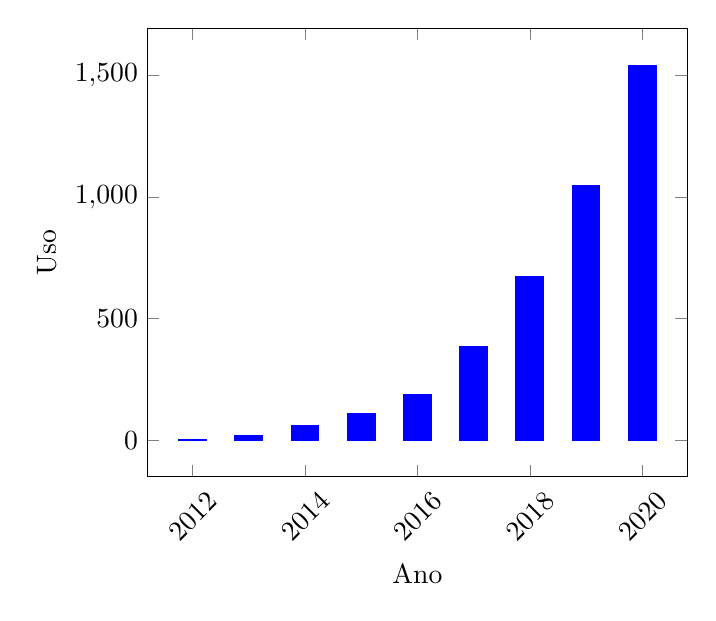
\begin{tikzpicture}[ybar]
		\begin{axis}[
				xlabel=Ano,ylabel=Uso,
				x tick label style={rotate=45, /pgf/number format/.cd,
						scaled x ticks = false,
						set thousands separator={},
						fixed}]
			\addplot [draw=blue, fill=blue] coordinates {
					(2012, 6)
					(2013, 19)
					(2014, 62)
					(2015, 113)
					(2016, 189)
					(2017, 387)
					(2018, 671)
					(2019, 1045)
					(2020, 1538)
				};
		\end{axis}
	\end{tikzpicture}
\end{frame}

\begin{frame}{\href{https://mc-stan.org}{\texttt{Stan}}\footnote{baseado no \href{https://breckbaldwin.github.io/ScientificSoftwareImpactMetrics/DeepLearningAndBayesianSoftware.html}{reporte anual do Breck Baldwin para a NUMFocus}}\footnote{veja as buscas Scopus nos \hyperlink{appendixscopus}{Slides de Backup no final dessa apresentação}}}
	\centering
	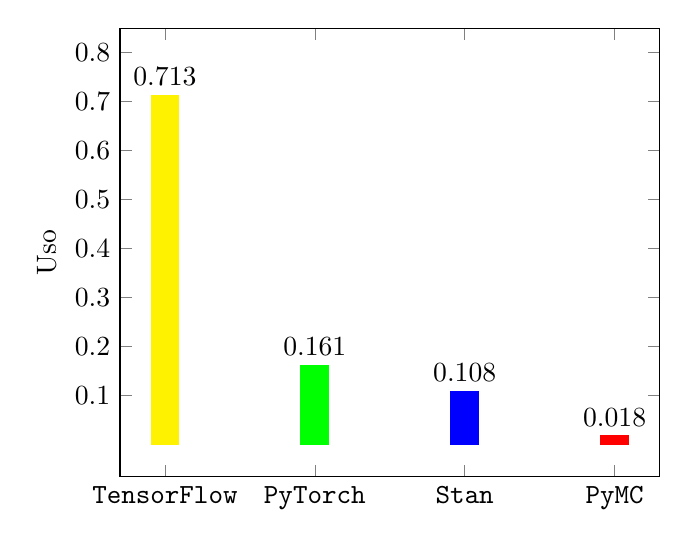
\begin{tikzpicture}[ybar]
		\begin{axis}[
				nodes near coords={\pgfmathprintnumber[fixed,precision=3]{\pgfplotspointmeta}},
				ylabel=Uso, xtick={1,2,3,4},
				ymax=0.85,
				ytick={0.1, 0.2, 0.3, 0.4, 0.5, 0.6, 0.7, 0.8},
				xticklabels={\texttt{TensorFlow}, \texttt{PyTorch}, \texttt{Stan}, \texttt{PyMC}}]
			\addplot [draw=yellow, fill=yellow] coordinates {
					(1, 0.713)};
			\addplot [draw=green, fill=green] coordinates {
					(2, 0.161)};
			\addplot [draw=blue, fill=blue] coordinates {
					(3, 0.108)};
			\addplot [draw=red, fill=red] coordinates {
					(4, 0.0176)};
		\end{axis}
	\end{tikzpicture}
\end{frame}

\subsection{Especificação de Modelos com Fórmulas}
\begin{frame}[fragile]{Especificação de Modelos com Fórmulas}
	Todos os modelos especificados pelo \href{http://mc-stan.org/rstanarm/}{\texttt{rstanarm}}
	e \href{https://paul-buerkner.github.io/brms/}{\texttt{brms}} usam uma fórmula
	com a seguinte síntaxe:
	\vfill
	\begin{lstlisting}
    dependente ~ independente_1 + independente_2 + ...
    \end{lstlisting}
\end{frame}

\begin{frame}[fragile]{Especificação de Modelos com Fórmulas}
	Moderações?! Sem problema:
	\vfill
	\begin{lstlisting}[basicstyle=\footnotesize]
dependente ~ independente_1 * moderadora + independente_2 * moderadora + ...
    \end{lstlisting}
\end{frame}

\subsection{Funções de Verossimilhança com \texttt{family}}
\begin{frame}{Funções de Verossimilhança com \texttt{family}}
	Todo modelo especificado pelo \href{http://mc-stan.org/rstanarm/}{\texttt{rstanarm}} e
	\href{https://paul-buerkner.github.io/brms/}{\texttt{brms}} devem especificar qual
	família da função de verossimilhança (\texttt{family}) respectivamente com a
	função de ligação (\texttt{link}) que fará o mapeamento dos parâmetros
	condicionados nos dados para a variável
	dependente\footnote{caso o usuário não designe nenhum valor para esses dois parâmetros, \href{http://mc-stan.org/rstanarm/}{\texttt{rstanarm}} e \href{https://paul-buerkner.github.io/brms/}{\texttt{brms}} usarão a verossimilhança Gaussiana (\texttt{family = gaussian}) e a função de identidade como função de ligação (\texttt{link = "identity"})}.
\end{frame}

\begin{frame}{Funções de Verossimilhança com \texttt{family}}
	\begin{vfilleditems}
		\item Gaussiana -- \texttt{family = gaussian(link = "identity")}
		\item Log-Normal -- \texttt{family = lognormal(link = "log")}
		\item Binomial -- \texttt{family = binomial(link = "logit")}
		\item Poisson -- \texttt{family = poisson(link = "log")}
		\item Binomial Negativa -- \texttt{family = negbinomial(link = "log")}
		\item $t$ de Student -- \texttt{family = student(link = "identity")}
		\item Exponencial -- \texttt{family = exponential(link = "log")}
	\end{vfilleditems}
\end{frame}

\subsection{\texttt{rstanarm}}

\begin{frame}{\href{http://mc-stan.org/rstanarm/}{\texttt{rstanarm}}\footnote{\textcite{rstanarm}}}
	O \href{http://mc-stan.org/rstanarm/}{\texttt{rstanarm}} é a porta de
	entrada para estatística Bayesiana com \href{https://mc-stan.org}{\texttt{Stan}}.
	\vfill
	O nome \texttt{rstanarm} é:
	\begin{vfilleditems}
		\item \texttt{r}: pacote para \texttt{R}
		\item \texttt{stan}: usa a linguagem probabilística \texttt{Stan}
		\item \texttt{arm}: acrônimo para \textit{Applied Regression Modeling}
	\end{vfilleditems}
\end{frame}

\subsubsection{Modelos do \texttt{rstanarm}}
\begin{frame}{Modelos do \href{http://mc-stan.org/rstanarm/}{\texttt{rstanarm}}\footnote{Neste curso usaremos apenas \texttt{stan\_glm} e \texttt{stan\_glmer}, mas saiba que você possui uma vasta categoria de modelos Bayesianos à disposição}}
	\begin{vfilleditems}
		\item \texttt{stan\_glm()} -- modelos lineares generalizados (\textit{\textbf{g}eneralized \textbf{l}inear \textbf{m}odel})
		\item \texttt{stan\_lm()} -- modelos lineares regularizados (\textit{\textbf{l}inear \textbf{m}odel)}
		\item \texttt{stan\_aov()} -- modelo ANOVA (\textit{\textbf{an}alysis \textbf{o}f \textbf{va}riance})
		\item \texttt{stan\_glmer()} - modelos linares generalizados multiníveis
		\item \texttt{stan\_lmer()} -- modelos linares regularizados multiníveis
		\item \texttt{stan\_jm()} -- modelos longitudinais e de sobrevivência
		\item \texttt{stan\_nlmer()} -- modelos não-lineares multiníveis (\textit{\textbf{n}on-\textbf{l}inear \textbf{m}odel})
		\item \texttt{stan\_polr()} -- modelos ordinais
		\item \texttt{stan\_gamm4()} -- modelos aditivos linares multiníveis
	\end{vfilleditems}
\end{frame}

\begin{frame}[fragile]{Exemplo Simples do \href{http://mc-stan.org/rstanarm/}{\texttt{rstanarm}}}
	\begin{lstlisting}
    library(rstanarm)
    rstanarm_fit <- @stan_glm(mpg ~ wt + am, data = mtcars)@
    summary(rstanarm_fit)
    \end{lstlisting}
\end{frame}

\begin{frame}{\texttt{summary} do \href{http://mc-stan.org/rstanarm/}{\texttt{rstanarm}}}
	\centering
	\begin{tabular}{lrrrrrrr}
		\toprule
		Parameter   & Rhat & n\_eff & mean  & sd   & 2.5\% & 50\%  & 97.5\% \\
		\midrule
		(Intercept) & 1.00 & 2157   & 37.16 & 3.20 & 30.78 & 37.16 & 43.44  \\
		wt          & 1.00 & 2285   & -5.32 & 0.83 & -6.91 & -5.32 & -3.65  \\
		am          & 1.00 & 2263   & 0.07  & 1.62 & -3.11 & 0.07  & 3.15   \\
		\bottomrule
	\end{tabular}
\end{frame}

\subsubsection{Visualizações do \texttt{rstanarm}}
\begin{frame}{Visualizações do \href{http://mc-stan.org/rstanarm/}{\texttt{rstanarm}}}
	% rstanarm_fit <- stan_glm(mpg ~ wt + am, data = mtcars)
	% library(ggplot2)
	% library(ggdark)
	% library(bayesplot)
	% library(tikzDevice)
	% theme_set(dark_theme_light())
	% bayesplot_theme_set(dark_theme_light())
	% tikz(file = "slides/images/mcmc_areas.tex")
	% mcmc_dens(rstanarm_fit)
	% dev.off()
	\centering
	\begin{figure}
		\resizebox{.45\linewidth}{!}{\input{images/mcmc_trace.tex}}
	\end{figure}
\end{frame}

\begin{frame}{Visualizações do \href{http://mc-stan.org/rstanarm/}{\texttt{rstanarm}}}
	% rstanarm_fit <- stan_glm(mpg ~ wt + am, data = mtcars)
	% library(ggplot2)
	% library(ggdark)
	% library(bayesplot)
	% library(tikzDevice)
	% theme_set(dark_theme_light())
	% bayesplot_theme_set(dark_theme_light())
	% tikz(file = "slides/images/mcmc_areas.tex")
	% mcmc_dens(rstanarm_fit)
	% dev.off()
	\centering
	\begin{figure}
		\resizebox{.45\linewidth}{!}{\input{images/mcmc_density.tex}}
	\end{figure}
\end{frame}

\subsubsection{Otimizações do \texttt{rstanarm}}
\begin{frame}{Otimizações do \href{http://mc-stan.org/rstanarm/}{\texttt{rstanarm}}}
	\begin{vfilleditems}
		\item Por padrão \href{http://mc-stan.org/rstanarm/}{\texttt{rstanarm}}
		usa \textbf{NCP}\footnote{\textit{Non-Centered Parameterization}}
		em \textbf{modelos multiníveis}\footnote{mais sobre isso quando falamos de modelos multiníveis}
		\item Por padrão \href{http://mc-stan.org/rstanarm/}{\texttt{rstanarm}}
		usa \textbf{centraliza as covariáveis em zero} para facilitar o trabalho do amostrador
		MCMC.
		\item Em modelos binomiais (regressão logística) é mais eficiente computacionalmente
		especificar uma fórmula usando o \lstinline!cbind! --
		\lstinline!stan_glm(cbind(successos, n - successos) ~ ...)!
		\item É possível especificar para que \href{http://mc-stan.org/rstanarm/}{\texttt{rstanarm}}
		use uma decomposição QR\footnote{veja os detalhes matemáticos nos \hyperlink{appendixqr}{Slides de Backup no final dessa apresentação}}
		da matrix de dados facilitando o trabalho do amostrador MCMC
		-- \lstinline!stan_glm(..., QR = TRUE)!
	\end{vfilleditems}
\end{frame}

\subsection{\texttt{brms}}
\begin{frame}{\href{https://paul-buerkner.github.io/brms/}{\texttt{brms}}\footnote{\textcite{brms}}}
	O \href{https://paul-buerkner.github.io/brms/}{\texttt{brms}} alia toda a
	comodidade do \href{http://mc-stan.org/rstanarm/}{\texttt{rstanarm}} com o
	poder e flexibilidade do \href{https://mc-stan.org}{\texttt{Stan}}.
	O nome \texttt{brms} quer dizer:
	\begin{vfilleditems}
		\item \texttt{b}: \textit{\textbf{b}ayesian}
		\item \texttt{r}: \textit{\textbf{r}egression}
		\item \texttt{m}: \textit{\textbf{m}odels}
		\item \texttt{s}: usando a linguagem probabilística \texttt{Stan}
	\end{vfilleditems}
\end{frame}
\subsubsection{Modelos do \texttt{brms}}
\begin{frame}{Modelos do \href{https://paul-buerkner.github.io/brms/}{\texttt{brms}}}
	Ao invés de possuir diversas funções para diferentes tipos de modelo,
	\texttt{brms} tem apenas uma única função para especificar modelos --
	\lstinline!brm(...)!
	\par
	O usuário consegue especificar qualquer modelo que quiser a partir da função
	\lstinline!brm(...)! apenas mudando seus parâmetros internos:
	\begin{vfilleditems}
		\item \lstinline!family! -- especifica a família da função de verossimilhança
		do modelo (padrão \lstinline!gaussian!)
		\item \lstinline!link! -- especifica a função de ligação
		que fará o mapeamento dos parâmetros condicionados nos dados para a variável
		dependente do modelo (padrão varia conforme o \lstinline!family!)
	\end{vfilleditems}
\end{frame}
\begin{frame}[fragile]{Exemplo Simples do \href{https://paul-buerkner.github.io/brms/}{\texttt{brms}}}
	\begin{lstlisting}
    library(brms)
    brms_fit <- @brm(mpg ~ wt + am, data = mtcars)@
    summary(brms_fit)
    \end{lstlisting}
\end{frame}

\begin{frame}{\texttt{summary} do \href{https://paul-buerkner.github.io/brms/}{\texttt{brms}}}
	\begin{table}[ht]
		\centering
		\begin{tabular}{lrrrrrrr}
			\toprule
			Parameter   & Rhat & n\_eff & mean  & sd   & 2.5\% & 50\%  & 97.5\% \\
			\midrule
			(Intercept) & 1.00 & 2361   & 37.28 & 3.22 & 30.83 & 37.30 & 43.79  \\
			wt          & 1.00 & 2486   & -5.35 & 0.83 & -7.03 & -5.35 & -3.71  \\
			am          & 1.00 & 2557   & -0.00 & 1.61 & -3.26 & 0.02  & 3.28   \\
			\bottomrule
		\end{tabular}
	\end{table}
\end{frame}
\subsubsection{Visualizações do \texttt{brms}}
\begin{frame}{Visualizações do \href{https://paul-buerkner.github.io/brms/}{\texttt{brms}}}
	% library(ggplot2)
	% library(ggdark)
	% library(bayesplot)
	% library(tikzDevice)
	% theme_set(dark_theme_light())
	% bayesplot_theme_set(dark_theme_light())
	% plot(conditional_effects(brms_fit, "wt"))
	% dev.off()
	% tikz(file = "slides/images/conditional_effects_am.tex")
	% plot(conditional_effects(brms_fit, "am"))
	% dev.off()
	\begin{columns}
		\begin{column}{0.5\textwidth}
			\centering
			\begin{figure}
				\resizebox{0.9\linewidth}{!}{\input{images/conditional_effects_wt.tex}}
			\end{figure}
		\end{column}
		\begin{column}{0.5\textwidth}
			\centering
			\begin{figure}
				\resizebox{0.9\linewidth}{!}{\input{images/conditional_effects_am.tex}}
			\end{figure}
		\end{column}
	\end{columns}
\end{frame}

\subsubsection{Otimizações do \texttt{brms}}
\begin{frame}{Otimizações do \href{https://paul-buerkner.github.io/brms/}{\texttt{brms}}}
	\small
	\begin{vfilleditems}
		\item Por padrão \href{https://paul-buerkner.github.io/brms/}{\texttt{brms}}
		\textbf{também} usa \textbf{NCP}\footnote{\textit{Non-Centered Parameterization}}
		em \textbf{modelos multiníveis}\footnote{mais sobre isso quando falamos de modelos multiníveis}
		\item Por padrão \href{https://paul-buerkner.github.io/brms/}{\texttt{brms}}
		\textbf{também} usa \textbf{centraliza as covariáveis em zero} para facilitar o trabalho do amostrador
		MCMC. Mas, você consegue desativar com \lstinline!bf(formula, center = FALSE)! sendo
		input da fórmula do \texttt{brms}
		\item Em modelos binomiais (regressão logística) é mais eficiente computacionalmente
		especificar uma fórmula usando o \lstinline!trials! --
		\lstinline!brms(success | trials(n) ~ ...)!
		\item É possível especificar para que \href{http://mc-stan.org/rstanarm/}{\texttt{rstanarm}}
		use uma decomposição QR\footnote{veja os detalhes matemáticos nos \hyperlink{appendixqr}{Slides de Backup no final dessa apresentação}}
		da matrix de dados facilitando o trabalho do amostrador MCMC
		-- \lstinline!bf(formula, decomp = "QR")! sendo input da fórmula do
		\texttt{brms}
	\end{vfilleditems}
\end{frame}

\begin{frame}[fragile]{\textit{Backend} \href{https://mc-stan.org/cmdstanr/}{\texttt{CmdStanR}} com o \href{https://paul-buerkner.github.io/brms/}{\texttt{brms}}}
	Além disso, \href{https://paul-buerkner.github.io/brms/}{\texttt{brms}} permite
	o uso de outros \textit{backend} além do \href{https://mc-stan.org/rstan/}{\texttt{RStan}}.
	\vfill
	Em especial o \href{https://mc-stan.org/cmdstanr/}{\texttt{CmdStanR}}
	sempre está mais atualizado que o \texttt{RStan} e tem algumas otimizações interessantes.
	Uma delas é o \lstinline!normalize! que usa o log PDF \textbf{não-normalizado} da função
	de verossimilhança, assim evitando computação de constantes ao usar o log PDF
	\textbf{normalizado} da função de verossimilhança\footnote{eu vejo, dependendo do modelo, um ganho de 25\% de velocidade}:
	\begin{lstlisting}
brm(..., backend = "cmdstanr", normalize = FALSE)
    \end{lstlisting}
\end{frame}
